\documentclass[11pt]{amsart}
\usepackage[
style=apa, natbib=true,
]{biblatex}
\addbibresource{biblio.bib} 
%prepared in AMSLaTeX, under LaTeX2e
\addtolength{\oddsidemargin}{-.75in} 
\addtolength{\evensidemargin}{-.75in}
\addtolength{\topmargin}{-.6in}
\addtolength{\textwidth}{1.4in}
\addtolength{\textheight}{1.3in}
\renewcommand{\baselinestretch}{1.06}

\usepackage{wrapfig,fancyvrb,xspace}
\usepackage{palatino,bm,stmaryrd}
\usepackage[final]{graphicx}
\usepackage[pdftex, colorlinks=true, plainpages=false, linkcolor=blue, citecolor=red, urlcolor=blue]{hyperref}

% macros
\newcommand{\bn}{\mathbf{n}}
\newcommand{\bq}{\mathbf{q}}
\newcommand{\bu}{\mathbf{u}}
\newcommand{\bv}{\mathbf{v}}
\newcommand{\bw}{\mathbf{w}}
\newcommand{\bx}{\mathbf{x}}

\newcommand{\bX}{\mathbf{X}}

\newcommand{\bsigma}{\bm{\sigma}}
\newcommand{\bomega}{\bm{\omega}}

\newcommand{\cH}{\mathcal{H}}
\newcommand{\cK}{\mathcal{K}}
\newcommand{\cT}{\mathcal{T}}
\newcommand{\cV}{\mathcal{V}}

\newcommand{\dx}{\mathrm{dx}}
\newcommand{\ds}{\mathrm{ds}}

\newcommand{\RR}{\mathbb{R}}

\newcommand{\Div}{\nabla\cdot}
\newcommand{\eps}{\epsilon}
\newcommand{\grad}{\nabla}
\newcommand{\lam}{\lambda}

\newcommand{\jump}[1]{\llbracket #1 \rrbracket }


\title{Gas in a porous media, using Firedrake}
\author{Tara Shreve}
\author{Ed Bueler}
\date{\today}

\begin{document}
\maketitle
%\begin{abstract}
%FIXME
%\end{abstract}

\thispagestyle{empty}

\section{A (draft) porous medium model for Darcy-type gas flow}

Suppose $\Omega$ is a 2-dimensional domain with well-behaved boundary, such as a rectangle or other polygon.  We will use $x$ for the horizontal and $z$, measured positive upward, for the vertical coordinate.  Within $\Omega$ we assume there is a matrix of porous material with spatially-variable porosity $\phi(x,z)$ and permeability $k(x,z)$, but these are assumed independent of time.  An ideal gas flows through the medium.  We will take various properties of this gas to be positive constants: $R$ is the gas constant, $T$ is the absolute temperature, and $M$ is the molar mass.  The ideal gas law then says the density $\rho$ and pressure $P$ are proportional:
\begin{equation}
RT \rho = M P.  \label{eq:ideal}
\end{equation}
Let $c = RT/M$, a positive constant.

We assume that the gas flow satisfies Darcy's law [REF?], driven by the deviation of gas pressure from the (litho)static distribution.  The lithostatic distribution is the pressure field $P_0=-\rho g z$ for which there would be no flow; here $g$ is the (constant) acceleration of gravity.  Thus
\begin{equation}
P-P_0 = c\rho+\rho g z \label{eq:drivingpressure}
\end{equation}
is the driving distribution, the pressure head.  Adding mass conservation, the following system of equations therefore applies to determing the evolution of the density $\rho(t,x,z)$, in SI units of $\text{kg}\,\text{m}^{-3}$, and (vector) volumetric flux $\bq(t,x,z)$, in units $\text{m}^3\,\text{m}^{-2}\,\text{s}^{-1} = \text{m}\,\text{s}^{-1}$:
\begin{subequations}
\label{eq:pmtime}
\begin{align}
\bq &= - \frac{k}{\mu} \grad\left(c \rho + \rho g z\right) \label{eq:pmtime:darcy} \\
\phi \frac{\partial \rho}{\partial t} + \Div \left(\rho\, \bq\right) &= 0. \label{eq:pmtime:masscont}
\end{align}
\end{subequations}
Here $\mu$ is the dynamic viscosity of the gas, again taken to be constant.

Several observations can be made.  To be physical the gas density must be non-negative: $\rho\ge 0$.  Relative to the classic mass continuity statement ``$\partial\rho/\partial t + \Div(\rho \bu)=0$'' \citep{Tadmor2012}, where $\bu$ is the fluid velocity, \eqref{eq:pmtime:masscont} is scaled with the porosity.  In fact this porosity is implicit in the definition of $\bq$ as a gas volume per unit area of (a face of) the porous matrix, equivalently $\bq$ is related to $\bu$ by $\bq = \phi \bu$, that is, via the dimensionless porosity.  Note that, while the velocity $\bu$ may be helpful in diagnosing the solution, it is not needed to state the model.

It is straightforward to eliminate the flux $\bq$ if desired:
\begin{equation}
\phi \frac{\partial \rho}{\partial t} - \Div \left(\frac{k}{\mu} \rho \grad\left(c \rho + \rho g z\right)\right) = 0. \label{eq:pmtime:primal}
\end{equation}
This form is comparable to the better-known heat equation
\begin{equation}
\frac{\partial u}{\partial t} - \Div(\grad u) = 0. \qquad \text{\emph{(heat equation)}}\label{eq:heattime:primal}
\end{equation}
An important property of \eqref{eq:heattime:primal} is that the operator $\Div \grad = \grad^2$ acts as an invertible matrix when finding the solution $u$.  However, since $\rho$ appears as a flux coefficient in \eqref{eq:pmtime:primal}, invertibility is lost if $\rho\to 0$ somewhere.  This ``degeneration'' of the diffusivity is a well-known property \citep{Vazquez2007} of the porous medium equation \eqref{eq:pmtime:primal}; it will influence the numerical solution method below.

System \eqref{eq:pmtime} is time dependent, but setting $\partial \rho/\partial t = 0$ yields the (mixed) strong form for the steady-state problem.  First we define the (conserved) mass flux in \eqref{eq:pmtime:masscont} as
\begin{equation}
\bsigma = \rho \bq, \label{eq:massflux}
\end{equation}
with units of $\text{kg}\,\text{m}^{-2}\,\text{s}^{-1}$.  Now we write the strong form in terms of the conserved density $\rho$ and its flux $\bsigma$:
\begin{subequations}
\label{eq:pm:strong}
\begin{align}
\bsigma &= - \frac{k}{\mu} \rho \grad\left(c \rho + \rho g z\right) \label{eq:darcy} \\
\Div \bsigma &= 0 \label{eq:masscont}
\end{align}
\end{subequations}
Not we are assuming no mass sources or sinks, as otherwise there would be a function on the right of \eqref{eq:masscont}.

Suitable boundary conditions must apply to system \eqref{eq:pm:strong}.  Along the ``Dirichlet'' part of the boundary, denoted $\Gamma_D \subset \partial\Omega$, the density (or pressure) is given.  On the remainder of the boundary $\Gamma_N = \partial\Omega \setminus \Gamma_D$, the ``Neumann'' boundary, the normal mass flux is zero. 
\begin{subequations}
\label{eq:strongbcs}
\begin{align}
\rho|_{\Gamma_D}               &= \rho_D(x,z) \\
(\bsigma\cdot \bn)|_{\Gamma_N} &= 0
\end{align}
\end{subequations}
It is easy to extend the model for provided values of the flux: $(\bsigma\cdot \bn)|_{\Gamma_N}= \sigma_N(x,z)$.

\section{Weak form allowing discontinuous permeability}

We will solve system \eqref{eq:pm:strong} by a conservative mixed finite element (FE) method \citep{Boffi2013}.  In this section we derive the weak form needed for this FE method via an element-wise weak form.  This derivation allows the permeability field to be discontinuous across element edges.

For the moment let $E$ be any well-behaved open subset of $\Omega$ with piecewise-$C^1$ boundary, and we assume that the exact, continuum solution $\bsigma$ and $\rho$ of \eqref{eq:pm:strong} are sufficiently continuous/smooth so that \eqref{eq:pm:strong} holds pointwise, which then allows the following derivation.  We multiply \eqref{eq:darcy} by a vector-valued test function $\bomega$, and \eqref{eq:masscont} by a scalar test function $v$, and integrate over $E$:
\begin{subequations}
\label{eq:pm:elementweak}
\begin{align}
\int_E \bsigma\cdot \bomega\,\dx + \int_E \frac{k}{\mu} \rho \grad\left(c \rho + \rho g z\right) \cdot \bomega\,\dx &= 0 \\
\int_E (\Div \bsigma) v\,\dx &= 0
\end{align}
\end{subequations}
Here $\dx = dx\,dz$ denotes the area integration element.  Also let $\ds$ denote the integration element over $\partial\Omega$ and $\bn$ the outward normal unit vector on $\partial E$.

The physical $k$ field is discontinuous.  For the FE method we will assume that the mesh edges include any such discontinuities of $k$.  Thus if $E$ is an element in the mesh, we will assume that all quantities in \eqref{eq:pm:elementweak}, and in the equations below, are continuous over $E$.  Also recall the divergence theorem
    $$\int_E \Div \bX\,\dx = \int_{\partial E} \bX\cdot \bn\,\ds$$
and the product rule $\Div(f\bX) = \grad f \cdot \bX + f \Div \bX$.  Then integration by parts uses these facts to remove the derivatives from the pressure head $c\rho+\rho g z$.  We get a new form
\begin{subequations}
\label{eq:elementweak:early}
\begin{align}
\int_E \bsigma\cdot \bomega\,\dx - \int_E \frac{1}{\mu} \left(c \rho + \rho g z\right) \Div(k\rho\bomega)\,\dx + \int_{\partial E} \frac{k}{\mu} \rho \left(c \rho + \rho g z\right) \bomega\cdot\bn\,\ds &= 0 \label{eq:elementweak:early:darcy} \\
\int_E (\Div \bsigma) v\,\dx &= 0 \label{eq:elementweak:early:masscont}
\end{align}
\end{subequations}

For convenience define the smooth field
\begin{equation}
C(z) = \frac{c + g z}{\mu},
\end{equation}
and also let
\begin{equation}
\hat\rho = \frac{1}{2}(\rho + |\rho|)  \label{eq:rhoplus}
\end{equation}
be the positive part of $\rho$.  Since $\hat\rho=\rho$ for the continuum solution, equation \eqref{eq:elementweak:early:darcy} is equivalent to
\begin{equation}
\int_E \bsigma\cdot \bomega\,\dx - \int_E C \hat\rho \Div(k\rho\bomega)\,\dx + \int_{\partial E} C \rho^2 \, k \bomega\cdot\bn\,\ds = 0 \label{eq:darcy:second}
\end{equation}

Now we sum equations \eqref{eq:darcy:second} and \eqref{eq:elementweak:early:masscont} over all elements $E$ in the mesh.  The mesh (triangulation), denoted $\cT_h$, is assumed to exactly cover the domain: $\bigcup_{E\in\cT_h} \bar E = \bar \Omega$.  Thus the original continuum solution also solves the following system:
\begin{subequations}
\label{eq:weak:early}
\begin{align}
\int_\Omega \bsigma\cdot \bomega\,\dx - \int_\Omega C \hat\rho \Div(k\rho\bomega)\,\dx + \sum_{E\in\cT_h} \int_{\partial E} C \rho^2 \, k \bomega\cdot\bn\,\ds &= 0 \label{eq:weak:early:darcy} \\
\int_\Omega (\Div \bsigma) v\,\dx &= 0 \label{eq:weak:early:masscont}
\end{align}
\end{subequations}

Let $\Gamma_0$ be the union of internal edges.  Then
\begin{equation}
\bigcup_{E\in\cT_h} \partial E = \Gamma_0 \cup \Gamma_D \cup \Gamma_N.
\end{equation}
Recalling boundary conditions \eqref{eq:strongbcs}, along $\Gamma_D$ the value $\rho=\rho_D$ is given.  The Neumann boundary condition is actually essential, so it involves a modification of the function space in which $\bsigma$ lives; the implementation is addressed below, but in any case these parts of the boundary interval vanish.  However, along edges in the internal boundary $\Gamma_0$ there are two elements adjacent to each edge.  Following standard conventions \citep{Arnold2002,Ham2023}, for each internal edge $e\in\Gamma_0$ there is an arbitrary choice of ``$+$'' and ``$-$'' adjacent elements.  Thus \eqref{eq:weak:early} becomes
\begin{subequations}
\label{eq:weak:second}
\begin{align}
\int_\Omega \bsigma\cdot \bomega\,\dx - \int_\Omega C \hat\rho \Div(k\rho\bomega)\,\dx + &\sum_{e\in\Gamma_0} \int_e \left(C_+ \rho_+^2 \, k_+ \bomega_+\cdot\bn_+ + C_- \rho_-^2 \, k_- \bomega_-\cdot\bn_-\right)\,\ds \label{eq:weak:second:darcy} \\
   &= -\int_{\Gamma_D} C \rho_D^2 \, k \bomega\cdot\bn\,\ds \notag \\
\int_\Omega (\Div \bsigma) v\,\dx &= 0 \label{eq:weak:second:masscont}
\end{align}
\end{subequations}

Based on experiments on the case of a linear Poisson equation with discontinuous coefficients, we believe that the internal edge integrals should be re-formulated as follows using standard notation \citep{Arnold2002}.  For a scalar function $f$ defined on the closure of each element let $\{f\} = \frac{1}{2} (f_+ + f_-)$ denote the average across the edge.  For a vector-valued function $\bv$ let $\jump{\bv} = \bv_+ \cdot \bn_+ + \bv_- \cdot \bn_-$ denote the jump across the edge, a scalar.  Then the quantities for which the continuum solution is expected to not have a jump are written as averages and the known jump in $k$ is explicitly stated.  The result is the weak form system which we plan to implement: 
\begin{subequations}
\label{eq:weak}
\begin{align}
\int_\Omega \bsigma\cdot \bomega\,\dx - \int_\Omega C \hat\rho \Div(k\rho\bomega)\,\dx + \sum_{e\in\Gamma_0} \int_e \{C \rho^2\} \jump{k \bomega}\,\ds &= -\int_{\Gamma_D} C \rho_D^2 \, k \bomega\cdot\bn\,\ds \label{eq:weak:darcy} \\
\int_\Omega (\Div \bsigma) v\,\dx &= 0 \label{eq:weak:masscont}
\end{align}
\end{subequations}


\section{Finite element implementation and solution}

FIXME implementation in which the flux $\bsigma$ is continuous across faces (edges) of the elements but the density distribution is approximated by a discontinuous scalar field

FIXME  On the remainder of the boundary we must impose the essential requirement that $\bomega\cdot \bn=0$ on the function space; this is done through Firedrake's \verb|DirichletBC()| command.

FIXME The first equation in this system weakly enforces Darcy's law and the second enforces conservation of mass.

FIXME To implement the above in Firedrake we must choose finite element spaces for $\bsigma$ and $\rho$.  To provide exact discrete mass conservation the vector fields $\bsigma$ should come from a space in which normal vectors are continuous across element boundaries.  The space for $\rho$ can be discontinuous.  Thus, for example, we may use the lowest-order Raviart-Thomas and DG pair which is stable for the mixed Poisson formulation:
\begin{Verbatim}[fontsize=\small,frame=lines]
S = FunctionSpace(mesh, 'RT', 1)
H = FunctionSpace(mesh, 'DG', 0)
W = S * H
w = Function(W)
sigma, rho = split(w)
omega, v = TestFunctions(W)
\end{Verbatim}
Weak form \eqref{eq:weak} then corresponds to the UFL code
\begin{Verbatim}[fontsize=\small,frame=lines]
FIXME
\end{Verbatim}
Here \verb|n = FacetNormal(mesh)|.  Note that \verb|ds(i)| requires indices \verb|i| for the appropriate boundary segments.

To solve the equations we apply Newton's method \citep{Kelley2003}.  Newton's method is managed by the SNES component of PETSc \citep{Balay2023}.  Some useful options are to use the default ``line search'' Newton solver \texttt{newtonls} but with the (non-default) back-tracking type of line search.  The linear Newton step equation are solved by a sparse direct matrix method \citep{Amestoy2001}.  Also we ask for feedback on the success or failure of the solver:
\begin{Verbatim}[fontsize=\small,frame=lines]
solve(F == 0, w, bcs=[BCs,],
      solver_parameters = {'snes_type': 'newtonls',
                           'snes_linesearch_type': 'bt',
                           'snes_rtol': 1.0e-5,
                           'snes_monitor': None,
                           'snes_converged_reason': None,
                           'ksp_type': 'preonly',
                           'pc_type': 'lu',
                           'pc_factor_mat_solver_type': 'mumps'})
\end{Verbatim}
A more advanced iterative, block-wise, and multigrid solver is possible \citep[e.g.][]{Bueler2021}, but it will require careful development.

Confirmation of global mass conservation is straightforward.  For example, on a rectangular domain with top side index \verb|4| and bottom side index \verb|3|:
\begin{Verbatim}[fontsize=\small,frame=lines]
topflux = assemble(dot(sigma,n) * ds(4))
bottomflux = assemble(dot(sigma,n) * ds(3))
imbalance = topflux + bottomflux
print(f'  flux out of top    = {topflux:13.6e}')
print(f'  flux into bottom   = {-bottomflux:13.6e}')
print(f'  imbalance          = {imbalance:13.6e}')
\end{Verbatim}
These \verb|assemble| expressions compute mass flux integrals
    $$\int_{\Gamma_i} \sigma\cdot \bn\,\ds = \int_{\Gamma_i} \rho \bq\cdot \bn\,\ds$$
over a particular side $\Gamma_i$.  In a typical run we get fluxes which balance to rounding error:
\begin{Verbatim}[fontsize=\small,frame=leftline]
FIXME
\end{Verbatim}


\section{An application for gas flow through a porous lava dome}

In \cite{Graham2023}, we measure permeability of samples from various textural units of the Obsidian dome and South Deadman dome using field and lab permeameters. These two domes are silicic lava flows in the Inyo Craters portion of the Mono-Inyo Craters in eastern California, a chain of silicic lava flows, domes, and explosion craters that stretches 12 km (7.5 miles) to the north-northeast of Long Valley Caldera. The Inyo craters erupted as recently as ~675 years (~1350 A.D.) before present. Prior studies subdivided the majority of the lava erupted at the Inyo Craters according to the observed vesicle textures found in different parts of each flow, subdivided into finely vesicular pumice (FV), coarsely vesicular pumice (CV), and dense obsidian (OB). Shallow scientific bore hole drilling in the 1970's confirmed the presence of an underground magmatic intrusion, which was the source of the domes. This drilling also provided some general constraints on the depth of each distinct textural unit within the dome (Table \ref{tab:UnitPermPoro}).

In this study, we wish to put constraints on the surface gas flux for each textural unit at Obsidian Dome. The unit mapping of the dome is shown in Fig. \ref{fig:unitMapping}, and an example cross-section is shown in Fig. \ref{fig:crossSection}. Using constraints on dome height, the depth and permeability of each unit, and assuming a significant portion of gas is sourced from degassing of the underlying feeder dike, we can use Darcy's law to calculate the surface gas flux through each unit. This was done in \cite{Graham2023} using a 1D model of Darcy's law, as implemented in \cite{Edmonds2003}, and we wish to extend this model into 2-dimensions, to account for the unit layering, which may affect the path of gas flow towards the surface.

COMSOL model results for gas density and surface gas flux are shown in Fig. \ref{fig:COMSOLresults}, with annotations stating relevant boundary conditions. Here we assume atmospheric pressure at the surface ($P_{atm} = 1.01325$ bar) and a pressure at the base of the dome ($L=22$ m) of $P_{z=L} = 11$ bar. There is a gas inlet at the base of the CV unit, through which steam at a temperature of 920$^{\circ}$C can enter the dome porous matrix. For simplicity, a no flow condition is imposed at the unit sides, and we choose to solve for the steady-state isothermal, compressible gas flow using Darcy's Law to relate volumetric gas flux and pressure. The porosity and permeability for each unit, as well as their height and percent of total dome surface area, are shown in Table \ref{tab:UnitPermPoro}.

\begin{figure}
   \centering
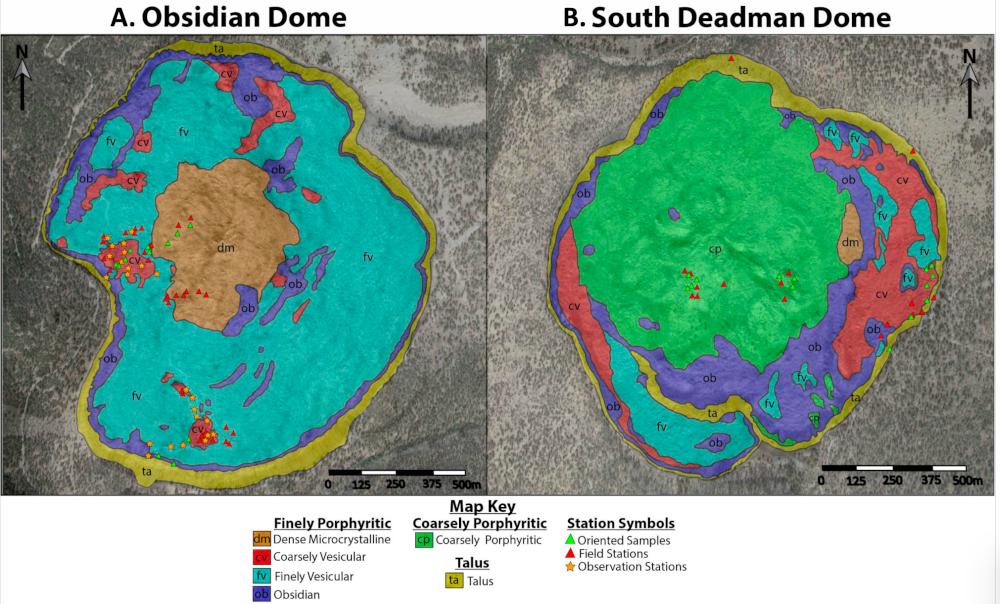
\includegraphics[width=0.95\textwidth]{figs/unitMapping-small.png}
\caption{Textural lithologic distribution maps of lavas for (A) Obsidian dome and (B) South Deadman dome.}
\label{fig:unitMapping}
\end{figure}

\begin{figure}
   \centering
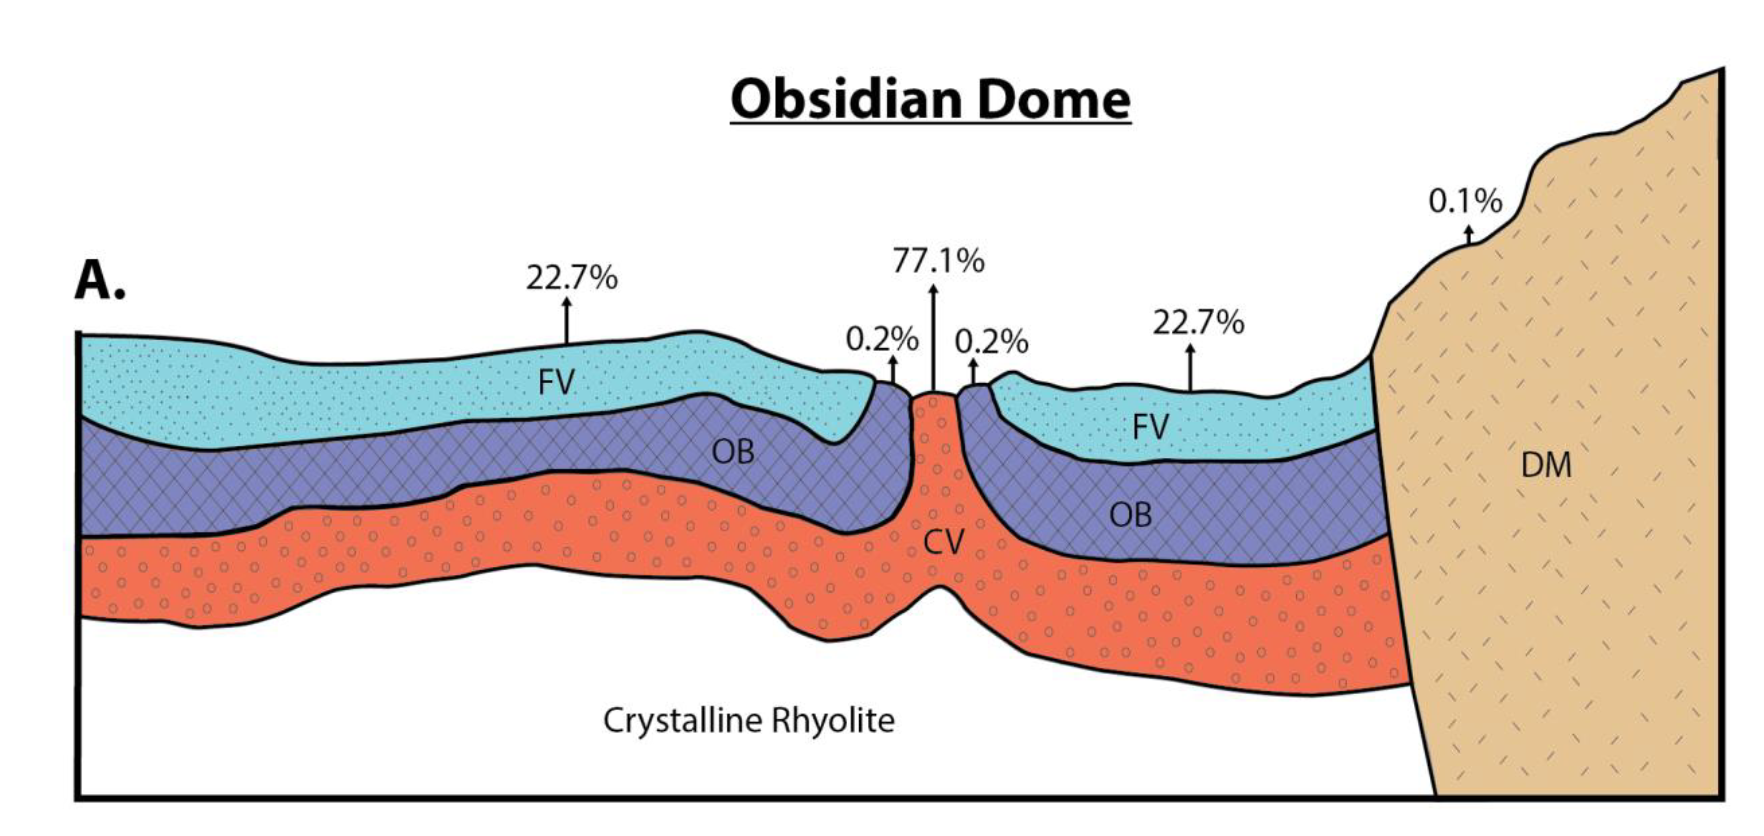
\includegraphics[scale=0.5]{figs/crossSection.png}
\caption{Schematic diagrams depicting total calculated gas flux percentages during the final stages of lava emplacement at Obsidian dome. Total gas flux for each lithologic unit was calculated using the gas flux model of Edmonds et al. (2003), and the gas flux percentages represent the percent gas flux for each lithologic unit relative to the total gas flux calculated for all units, and does not consider additional degassing that occurs through conduit processes, fractures, tuffisite veins, or porous pathways that are too large to measure.}
\label{fig:crossSection}
\end{figure}

\begin{figure}
   \centering
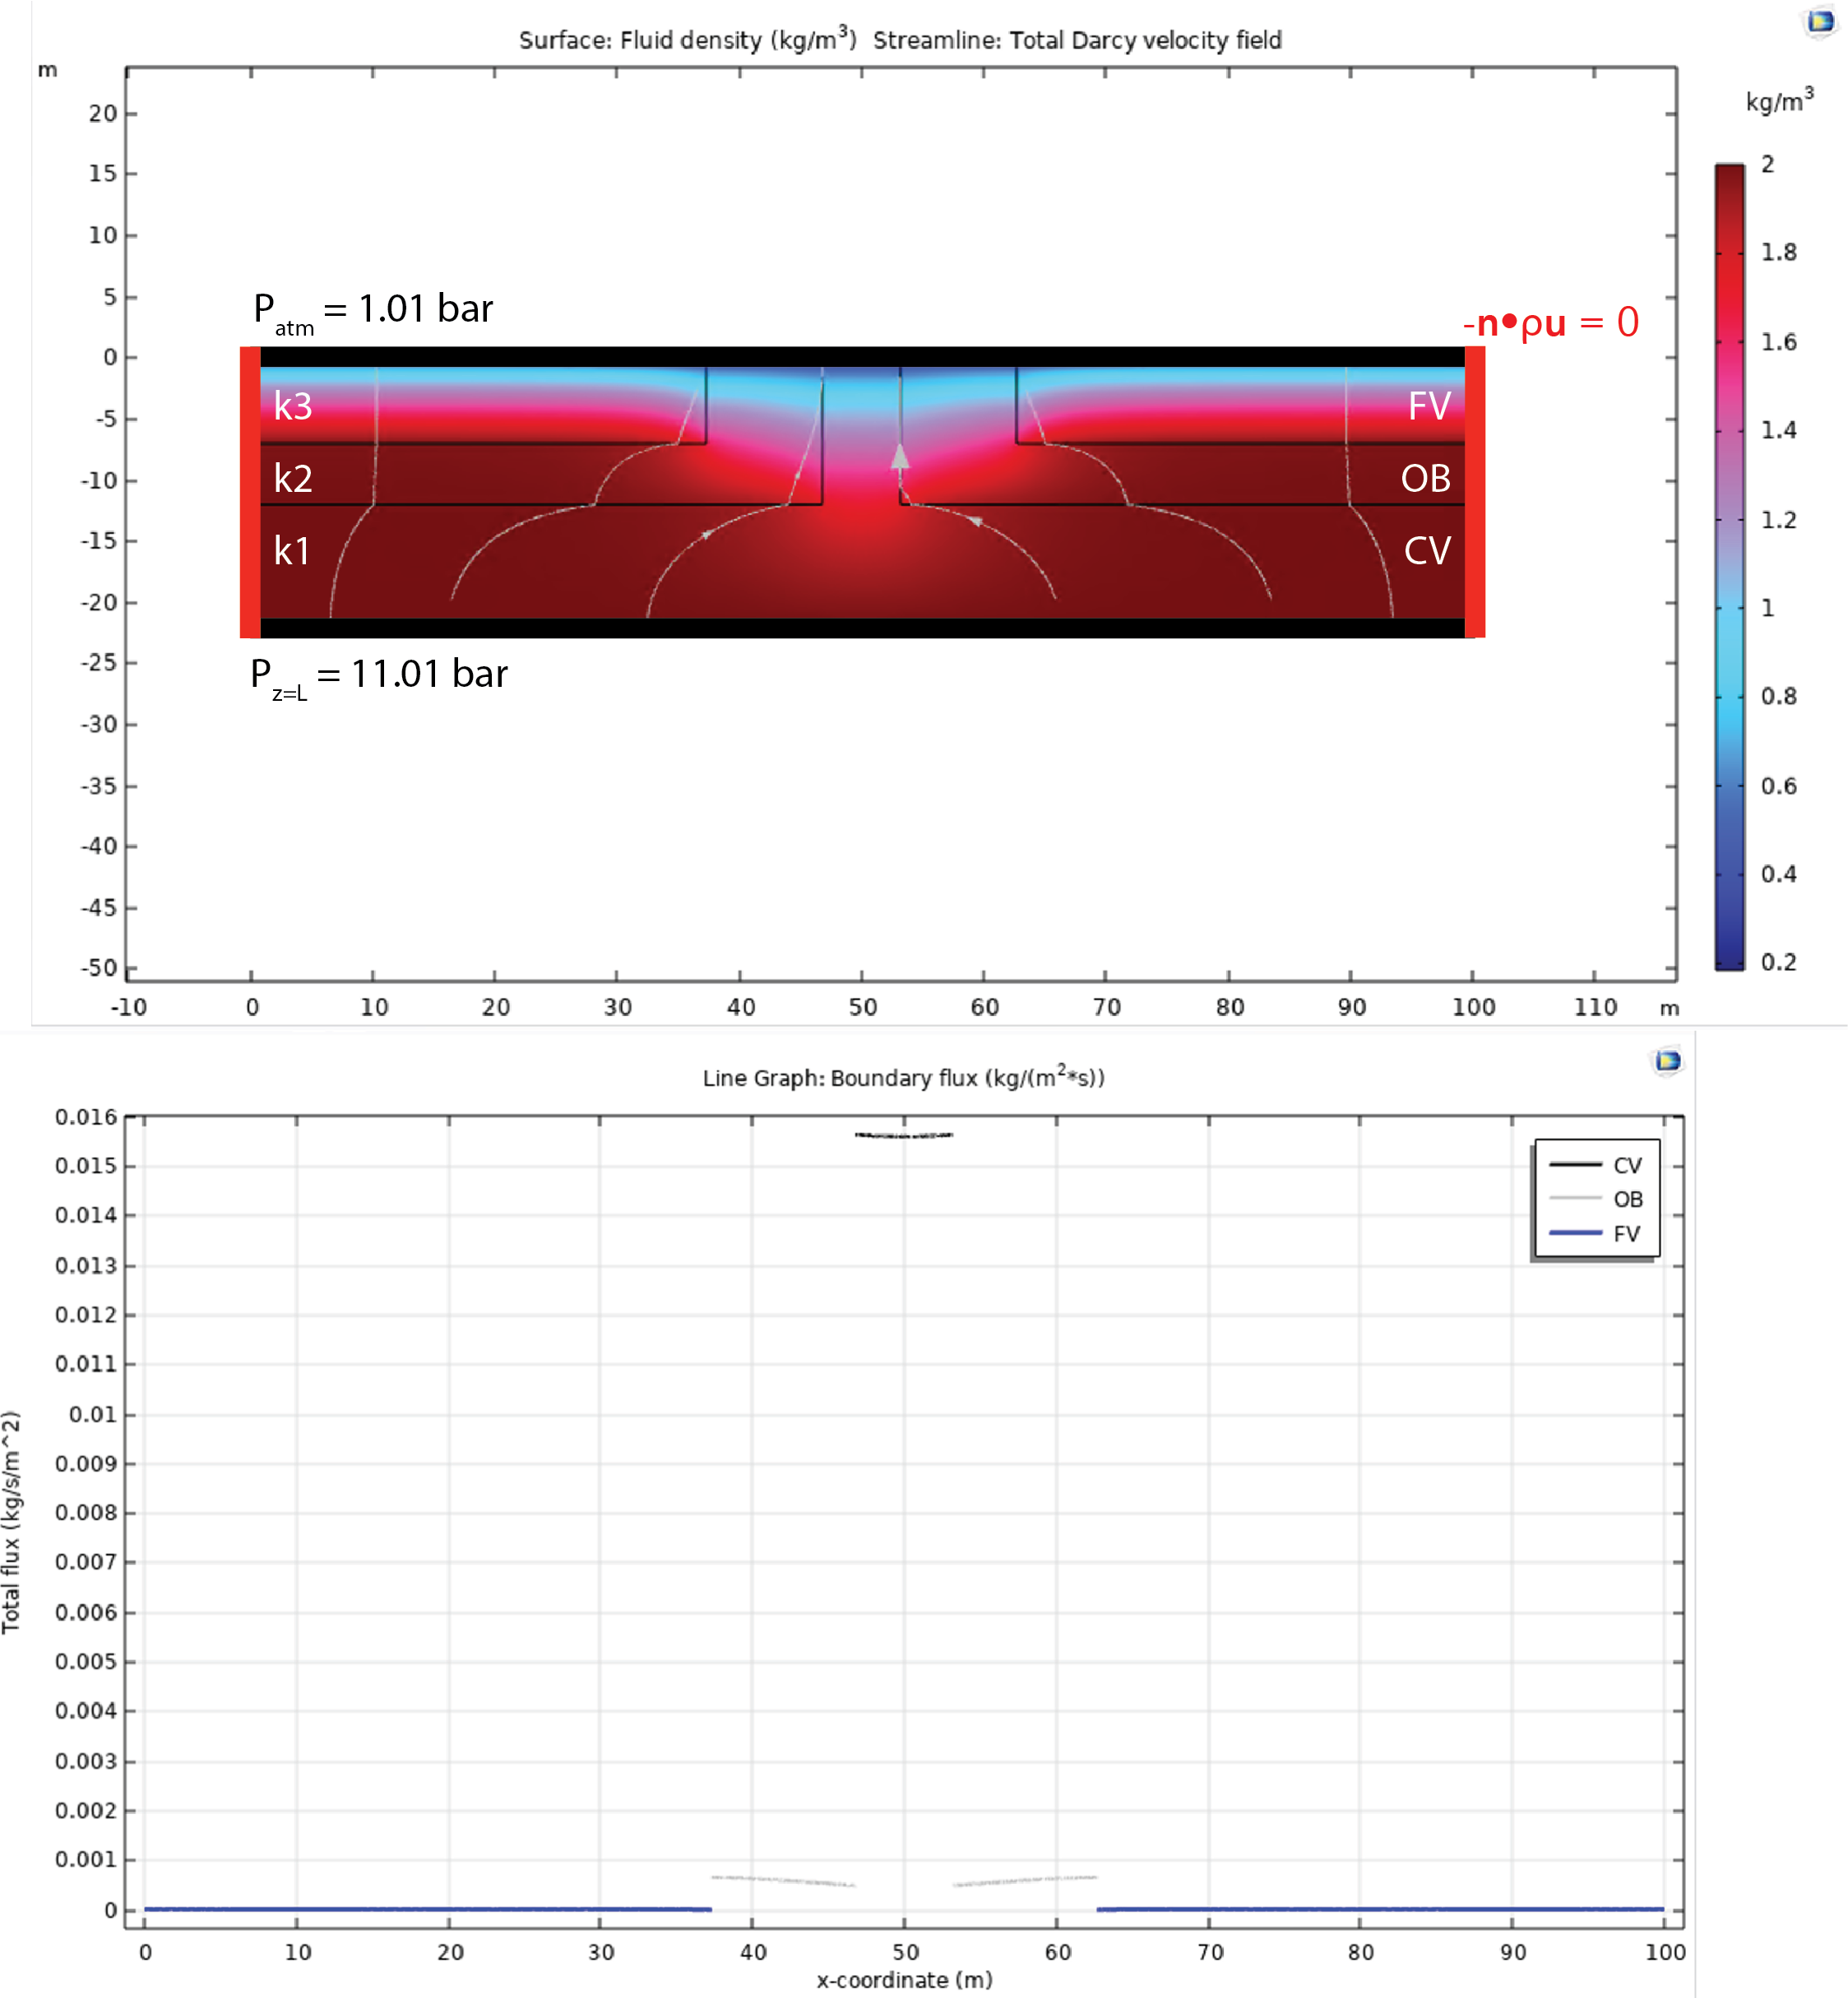
\includegraphics[scale=0.8]{figs/comsolDarcyLaw_units.png}
\caption{Top figure shows gas density in unit layers CV, FV, and OB, with permeabilities k1, k2, and k3, respectively (see Table \ref{tab:UnitPermPoro}). Streamlines indicate the direction of gas flow. Pressure boundary conditions at the base and surface of the units are shown in black, and no flow boundary conditions at the side of the units are shown in red. The bottom figure shows the gas flux at the surface.}
\label{fig:COMSOLresults}
\end{figure}


\begin{table}[h]
\center
      \small
      \begin{tabular}{lllll}
      \hline
      \textbf{Unit} & \textbf{Permeability (m\textsuperscript{2})} & \textbf{Connected porosity (\%)}  & \textbf{Height (m)} & \textbf{Percent of total dome surface area} \\  
      \hline
      CV & 6.87E-12 & 50.0 & 10 & 6.4 \\
      FV & 2.18E-13 & 23.2 &  7 & 74.6 \\
      OB & 4.94E-15 & 3.24 & 5 & 19.0 \\ 
\end{tabular}%}
\caption{Average permeability, porosity, height, and percent of total dome surface area of each textural unit.} 
\label{tab:UnitPermPoro}
\end{table}

\printbibliography

\end{document}
